A model written using a modeling language like Alloy is useful to understand better the problem and to check if the modeling of the problem is correct or needs to be refined. Alloy generates some instances starting from the model code in order to catch modeling errors. Fixing these errors in the early stages of the system lifecycle will cost a lot less than fixing them at later stages of the development cycle.

\subsection{Goals of the model}
The Alloy model proposed in the next subsection of this document will focus on the formalization of the queueing of the customers and the slot booking system. This model is static, meaning that each instance generated from the alloy engine depicts the state of the system in a given instant of the time. The goal of a static model is to generate instances from that model, these instances represent only the states that the system could assume the transition between these state are instead described from a dynamic model. Finding an invalid state means that something is wrong in the system or in the model, but if all states analyzed are correct this will not mean that the system static model is correct.
\subsection{Alloy Code}

\lstinputlisting[language=alloy]{alloy/model.als}
\clearpage
\subsection{Instance Analysis}
In this section some instances generated from the alloy engine will be shown in order to explain better the model.
For clarity some atoms and some relations between them are hidden. 
\begin{figure}[H]
    \hspace*{3.0cm}
    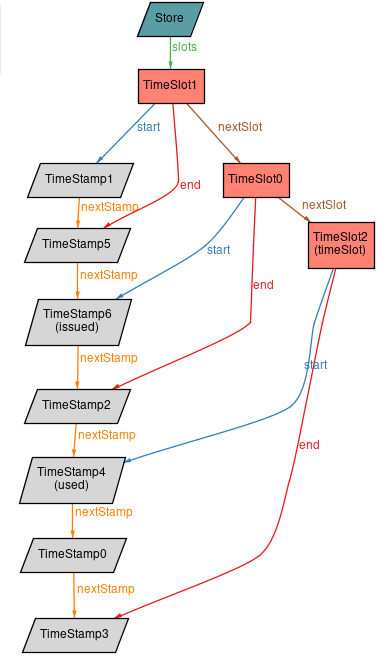
\includegraphics[scale=1.0]{Images/alloy_1_slots.png}
    \caption{\label{fig:Alloy_1}Instance diagram showing the Time Slots}
\end{figure}    

As shown in the Figure~\ref{fig:Alloy_1} the continuos time is modeled using discrete ordered timestamps. A timestamp is an instant of time when something relevant for the system happens (i.e. a time slot starts, a ticket is issued or used to enter the store). Each instance offers a view of a valid system state at the last (largest) timestamp, that in the first instance is TimeStamp0.

\pagebreak

In the Figure~\ref{fig:Alloy_1} instance diagram time slots atoms are shown. Every couple of time slots created from the same store must not overlap and the next time slot should start after the end of the current one.


\begin{figure}[H]
    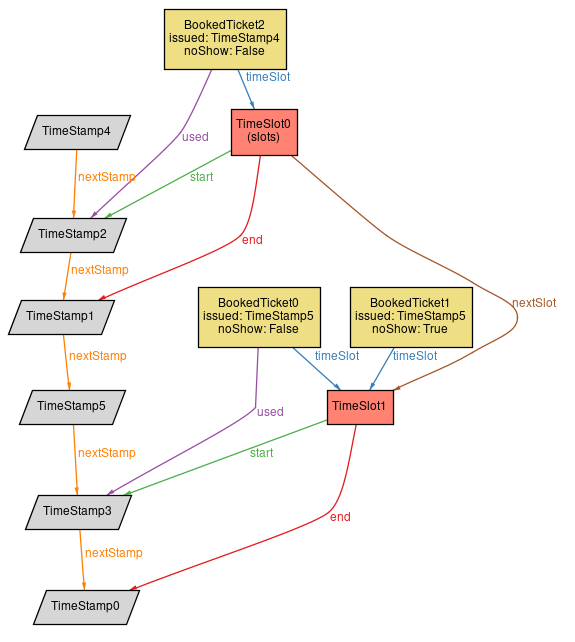
\includegraphics[width=\textwidth]{Images/alloy_3_booked.png}
    \caption{\label{fig:Alloy_2}Instance diagram showing Booked Tickets}
\end{figure}
In the Figure~\ref{fig:Alloy_2} booked tickets are shown in the diagram. Booked Tickets are a special type of ticket that are bound to a time slot. A Booked Ticket must be issued before the start of the time slot, and it has to be used within its time slot. A Booked Ticket not used in the bounded TimeSlots counts as a no-show ticket (representing the customer that books a ticket but does not show to the store in time).

\begin{figure}[H]
    \hspace*{2.8cm}
    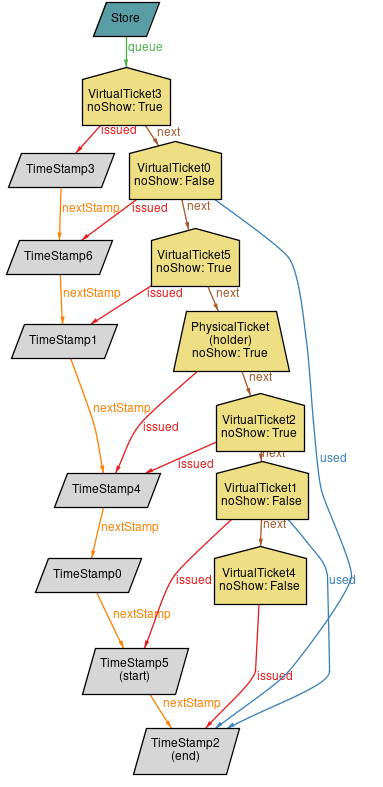
\includegraphics[]{Images/alloy_2_queue.png}
    \caption{\label{fig:Alloy_3}Instance diagram showing the queueing system}
\end{figure}

The Figure~\ref{fig:Alloy_3} explains how the store queueing system is modeled. If a customer doesn't book a ticket for entering in the store they have to retrieve a Numbered Ticket, either Virtual (using the application) or Physical (using the ticket emitter). These tickets are handed using a First Come First Served Logic, a ticket with a lower timestamp should be called to the entrance before a ticket with an higher one, and the timestamp when the ticket is used should reflect this order unless no-shows happen (i.e. A Customer that retrieves a ticket and then does not show when called to the entrance).